%% abtex2-modelo-projeto-pesquisa.tex, v-1.9.7 laurocesar
%% Copyright 2012-2018 by abnTeX2 group at http://www.abntex.net.br/ 
%%
%% This work may be distributed and/or modified under the
%% conditions of the LaTeX Project Public License, either version 1.3
%% of this license or (at your option) any later version.
%% The latest version of this license is in
%%   http://www.latex-project.org/lppl.txt
%% and version 1.3 or later is part of all distributions of LaTeX
%% version 2005/12/01 or later.
%%
%% This work has the LPPL maintenance status `maintained'.
%% 
%% The Current Maintainer of this work is the abnTeX2 team, led
%% by Lauro César Araujo. Further information are available on 
%% http://www.abntex.net.br/
%%
%% This work consists of the files abntex2-modelo-projeto-pesquisa.tex
%% and abntex2-modelo-references.bib
%%

% ------------------------------------------------------------------------
% ------------------------------------------------------------------------
% abnTeX2: Modelo de Projeto de pesquisa em conformidade com 
% ABNT NBR 15287:2011 Informação e documentação - Projeto de pesquisa -
% Apresentação 
% ------------------------------------------------------------------------ 
% ------------------------------------------------------------------------

\documentclass[
	% -- opções da classe memoir --
	12pt,				% tamanho da fonte
	openright,			% capítulos começam em pág ímpar (insere página vazia caso preciso)
	oneside,			% para impressão em recto e verso. Oposto a oneside
	a4paper,			% tamanho do papel. 
	% -- opções da classe abntex2 --
	%chapter=TITLE,		% títulos de capítulos convertidos em letras maiúsculas
	%section=TITLE,		% títulos de seções convertidos em letras maiúsculas
	%subsection=TITLE,	% títulos de subseções convertidos em letras maiúsculas
	%subsubsection=TITLE,% títulos de subsubseções convertidos em letras maiúsculas
	% -- opções do pacote babel --
	english,			% idioma adicional para hifenização
	french,				% idioma adicional para hifenização
	spanish,			% idioma adicional para hifenização
	brazil,				% o último idioma é o principal do documento
	]{abntex2}

% ---
% PACOTES
% ---

% ---
% Pacotes fundamentais 
% ---
\usepackage{lmodern}			% Usa a fonte Latin Modern
\usepackage[T1]{fontenc}		% Selecao de codigos de fonte.
\usepackage[utf8]{inputenc}		% Codificacao do documento (conversão automática dos acentos)
\usepackage{indentfirst}		% Indenta o primeiro parágrafo de cada seção.
\usepackage{color}				% Controle das cores
\usepackage{graphicx}			% Inclusão de gráficos
\usepackage{microtype} 			% para melhorias de justificação
% \usepackage{placeins}
\usepackage{listings}
\usepackage{color}
\usepackage{amsmath}

\usepackage{placeins}

\let\Oldsection\section
\renewcommand{\section}{\FloatBarrier\Oldsection}

\let\Oldsubsection\subsection
\renewcommand{\subsection}{\FloatBarrier\Oldsubsection}

\let\Oldsubsubsection\subsubsection
\renewcommand{\subsubsection}{\FloatBarrier\Oldsubsubsection}

\definecolor{dkgreen}{rgb}{0,0.6,0}
\definecolor{gray}{rgb}{0.5,0.5,0.5}
\definecolor{mauve}{rgb}{0.58,0,0.82}
% ---

% ---
% Pacotes adicionais, usados apenas no âmbito do Modelo Canônico do abnteX2
% ---
\usepackage{lipsum}				% para geração de dummy text
% ---

% ---
% Pacotes de citações
% ---
\usepackage[brazilian,hyperpageref]{backref}	 % Paginas com as citações na bibl
\usepackage[alf]{abntex2cite}	% Citações padrão ABNT

% --- 
% CONFIGURAÇÕES DE PACOTES
% --- 


% ---
% Configurações do pacote backref
% Usado sem a opção hyperpageref de backref
\renewcommand{\backrefpagesname}{Citado na(s) página(s):~}
% Texto padrão antes do número das páginas
\renewcommand{\backref}{}
% Define os textos da citação
\renewcommand*{\backrefalt}[4]{
	\ifcase #1 %
		Nenhuma citação no texto.%
	\or
		Citado na página #2.%
	\else
		Citado #1 vezes nas páginas #2.%
	\fi}%
% ---
\newcommand{\simpletext}{\noindent\ignorespaces\par\noindent\ignorespacesafterend}

% ---
% Informações de dados para CAPA e FOLHA DE ROSTO
% ---
\titulo{CLASSIFICAÇÃO DE PRODUTOS NO E-COMMERCE UTILIZANDO DADOS HETEROGÊNEOS}
\autor{Allan Batista \\ Victor Nascimento \\ Rodrigo Peres}
\local{Rio de Janeiro}
\data{2020, v-1.0.0}
\instituicao{%
  B2W Digital
  \par
  Pesquisa e desenvolvimento
%   \par
%   Programa de Pós-Graduação}
}
\tipotrabalho{Pesquisa e desenvolvimento}
% O preambulo deve conter o tipo do trabalho, o objetivo, 
% o nome da instituição e a área de concentração 
\preambulo{Trabalho de pesquisa e desenvolvimento na B2W Digital para a classificação de Produtos no e-commerce.}
% ---

% ---
% Configurações de aparência do PDF final

% alterando o aspecto da cor azul
\definecolor{blue}{RGB}{41,5,195}

% informações do PDF
\makeatletter
\hypersetup{
     	%pagebackref=true,
		pdftitle={\@title}, 
		pdfauthor={\@author},
    	pdfsubject={\imprimirpreambulo},
	    pdfcreator={LaTeX with abnTeX2},
		pdfkeywords={aprendizado de máquina}{redes neurais profundas}{redes convolucionais}{arquitetura transformer}, 
		colorlinks=true,       		% false: boxed links; true: colored links
    	linkcolor=blue,          	% color of internal links
    	citecolor=blue,        		% color of links to bibliography
    	filecolor=magenta,      	% color of file links
		urlcolor=blue,
		bookmarksdepth=4
}
\makeatother
% --- 

% --- 
% Espaçamentos entre linhas e parágrafos 
% --- 

% O tamanho do parágrafo é dado por:
\setlength{\parindent}{1.3cm}

% Controle do espaçamento entre um parágrafo e outro:
\setlength{\parskip}{0.2cm}  % tente também \onelineskip

% ---
% compila o indice
% ---
\makeindex
% ---

% ----
% Início do documento
% ----
\begin{document}

% Seleciona o idioma do documento (conforme pacotes do babel)
%\selectlanguage{english}
\selectlanguage{brazil}

% Retira espaço extra obsoleto entre as frases.
\frenchspacing 

% ----------------------------------------------------------
% ELEMENTOS PRÉ-TEXTUAIS
% ----------------------------------------------------------
% \pretextual

% ---
% Capa
% ---
\let\cleardoublepage=\clearpage
\imprimircapa
\let\cleardoublepage=\clearpage
% ---

% ---
% Folha de rosto
% ---
\imprimirfolhaderosto
\clearpage
% ---

% resumo em português
\begin{resumo}

A classificação de produtos no \textbf{e-commerce} é um desafio devido a sua variabilidade e qualidade das informações disponíveis. Este trabalho propõem uma arquitetura híbrida de \textbf{Rede Neural Artificial Profunda} para \textbf{dados heterogêneos e não estruturados} (texto e imagem) em uma única arquitetura que combina \textbf{Redes Neurais Convolucionais} e \textbf{Arquitetura “Transformer”} com uma estrutura de \textbf{classificação multinível}.

\vspace{\onelineskip}
 
\noindent
\textbf{Palavras-chave}: aprendizado de máquina, redes neurais profundas, redes convolucionais, arquitetura transformer.

\end{resumo}

% ---
% inserir lista de ilustrações
% ---
\pdfbookmark[0]{\listfigurename}{lof}
\listoffigures*
\clearpage
% ---

% ---
% inserir lista de tabelas
% ---
\pdfbookmark[0]{\listtablename}{lot}
\listoftables*
\clearpage
% ---

% ---
% inserir lista de abreviaturas e siglas
% ---
% \begin{siglas}
%   \item[BLAH] bla bla bla
% \end{siglas}
% ---

% ---
% inserir lista de símbolos
% ---
% \begin{simbolos}
%   \item[$ \Gamma $] Letra grega Gama
%   \item[$ \Lambda $] Lambda
%   \item[$ \zeta $] Letra grega minúscula zeta
%   \item[$ \in $] Pertence
% \end{simbolos}
% ---

% ---
% inserir o sumario
% ---
\pdfbookmark[0]{\contentsname}{toc}
\tableofcontents*
\clearpage
% ---


% ----------------------------------------------------------
% ELEMENTOS TEXTUAIS
% ----------------------------------------------------------
\textual


\chapter[Introdução]{Introdução}

Com continuo crescimento do e-commerce no Brasil nos últimos anos e a adesão cada vez maior de novas lojas no Marketplace, traz consigo um aumento considerável na entrada de novos produtos no site da companhia. Tal confirmação pode ser observado na \autoref{quantidade_de_produtos_por_mes}.

\begin{figure}[htb]
	\caption{\label{quantidade_de_produtos_por_mes} Quantidade de Produtos ao longo dos Meses 2018+}
	\begin{center}
	    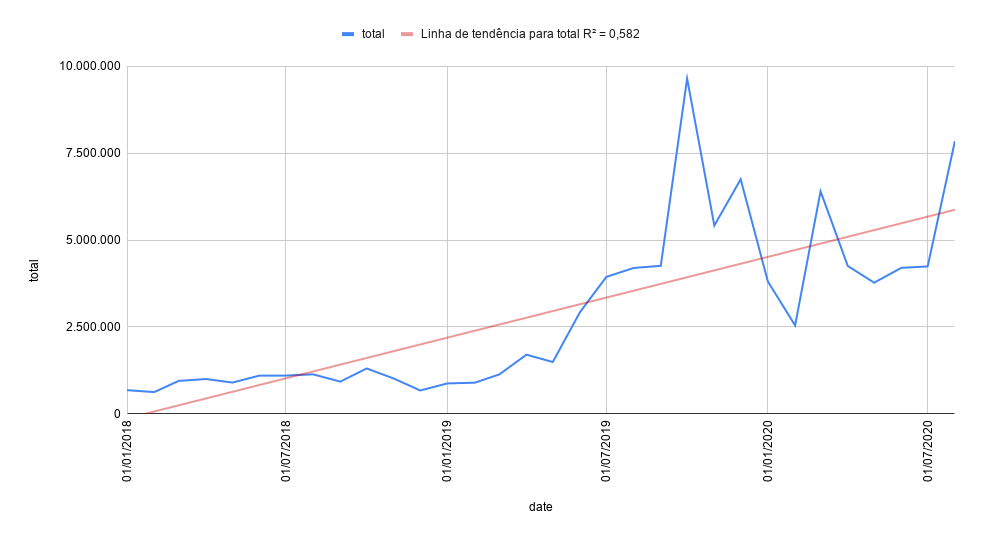
\includegraphics[width=\textwidth]{artigo/recursos/imagens/Quantidade de Produtos ao longo dos Meses 2018+.png}
	\end{center}
	\legend{Fonte: Elaborado pelo Autor}
\end{figure}

Quando os produtos entram no marketplace, eles precisam ser categorizados à fim de proporcionar uma melhor qualidade do catálogo ao cliente final ao buscar um produto no site. No entanto, existe uma quantidade expressiva de categorias, que pode ser observado na \autoref{tab:quantidade_de_categorias}, o que gera muita confusão e erros das lojas ao  categorizar um produto na estruturas das categorias.

\begin{table}[]
    \centering
    \caption{Quantidade de Categorias}
    \begin{tabular}{r|l} \hline
        Departamento & 60  \\ \hline
        Setor & 1152 \\ \hline
        Família & 4595 \\ \hline
        Subfamília & 8885 \\ \hline
    \end{tabular}
    \legend{Fonte: Elaborado pelo Autor}
    \label{tab:quantidade_de_categorias}
\end{table}

Portanto, se faz necessário a criação de um sistema capaz de fazer esta categorização de forma automática a fim de reduzir o custo, tempo e elevar a assertividade da classificação de produtos na entrada de novos itens no marketplace. 

Para a resolução deste problema, foi desenvolvido uma arquitetura de Redes Neurais Artificiais utilizando dados heterogêneos não estruturados (texto e imagem) dos produtos a fim de tornar a classificação mais eficiente do ponto de vista de assertividade.

\section{PORQUE UTILIZAR TEXTO E IMAGEM}

A necessidade de utilizar dois tipos de dados tão distintos durante a classificação, se faz necessário devido em alguns casos esses dados individualmente não possuírem informação o suficiente para classificar adequadamente a categoria do produto. Pode ser visto um exemplo de ambiguidade de produtos na \autoref{produtos_similares} em categorias distintas.

\begin{figure}[htb]
	\caption{\label{produtos_similares} Produtos similares em categorias distintas}
	\begin{center}
	    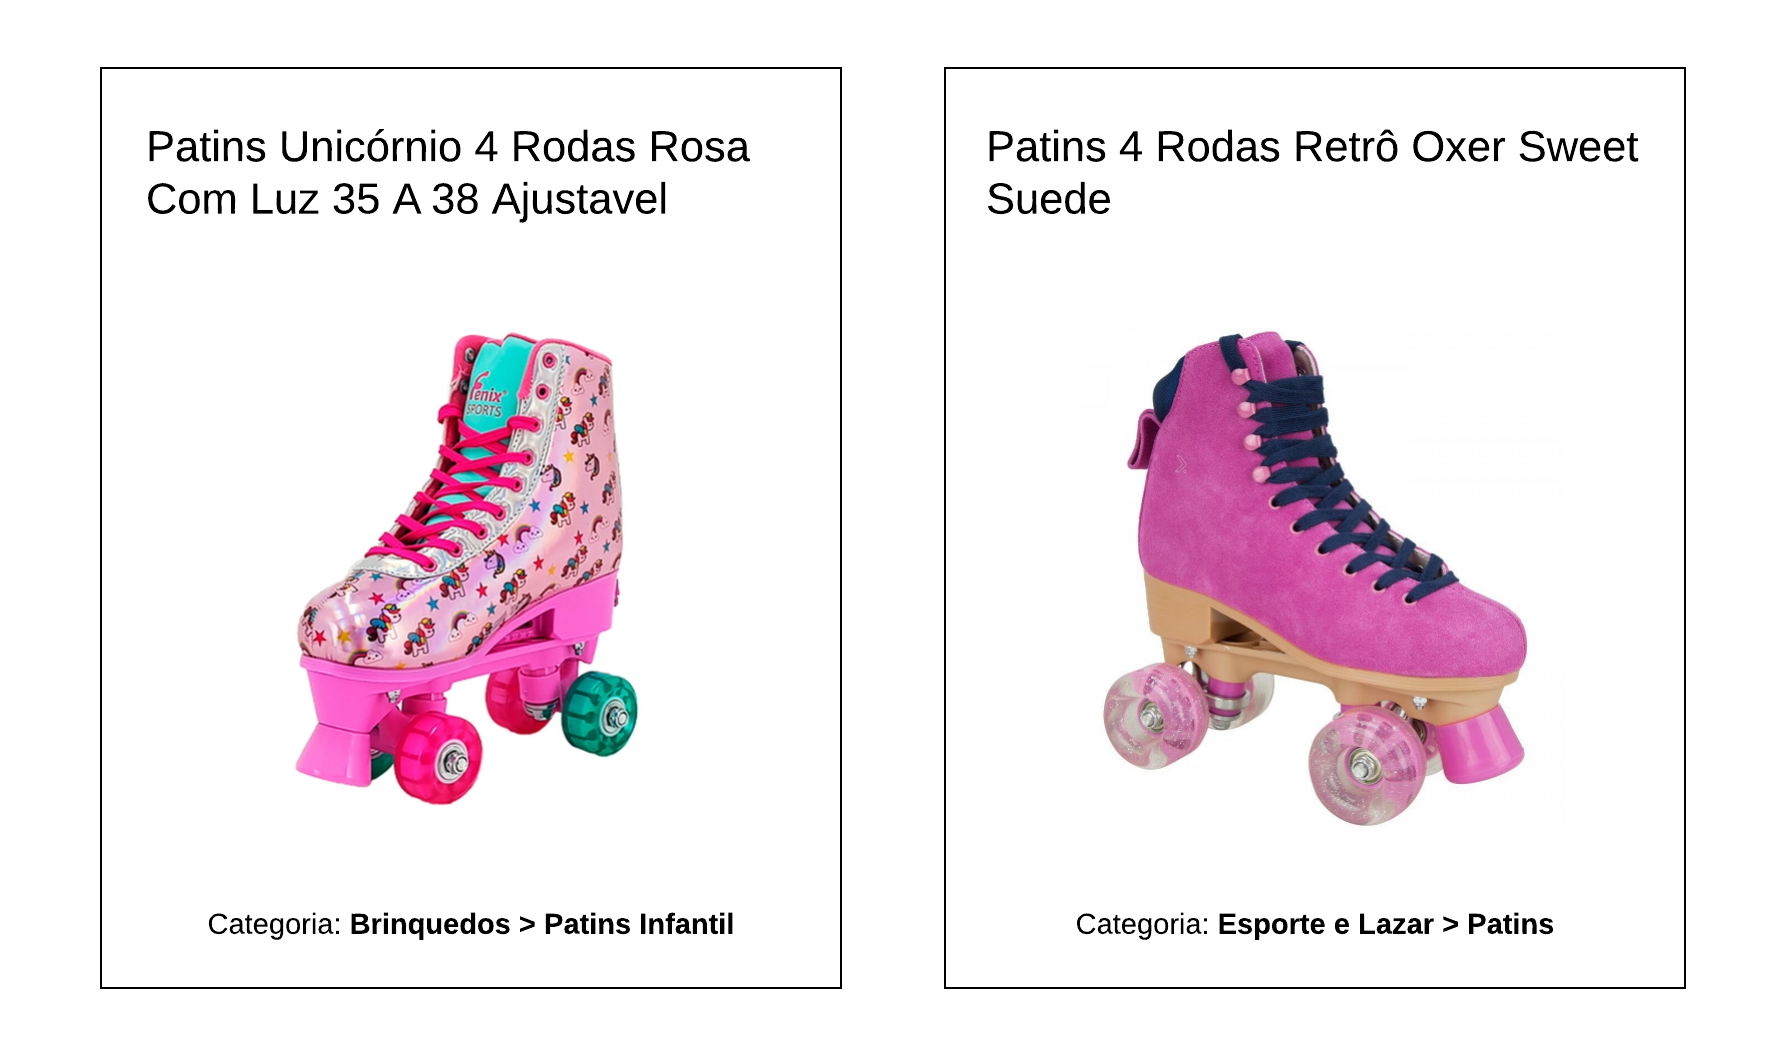
\includegraphics[scale=0.5]{artigo/recursos/imagens/produtos-similares.png}
	\end{center}
	\legend{Fonte: Elaborado pelo Autor}
\end{figure}

\section{ESTRUTURA DAS CATEGORIAS}

A estrutura das categorias é em formato de árvore e pode ser visto na \autoref{arvore_de_categorias}, onde os níveis superiores são mais genéricos enquanto os níveis mais baixos são mais específicos. Hoje existe um conjunto total de 14692 categorias.

\begin{figure}[htb]
	\caption{\label{arvore_de_categorias} Estrutura das categorias em árvore}
	\begin{center}
	    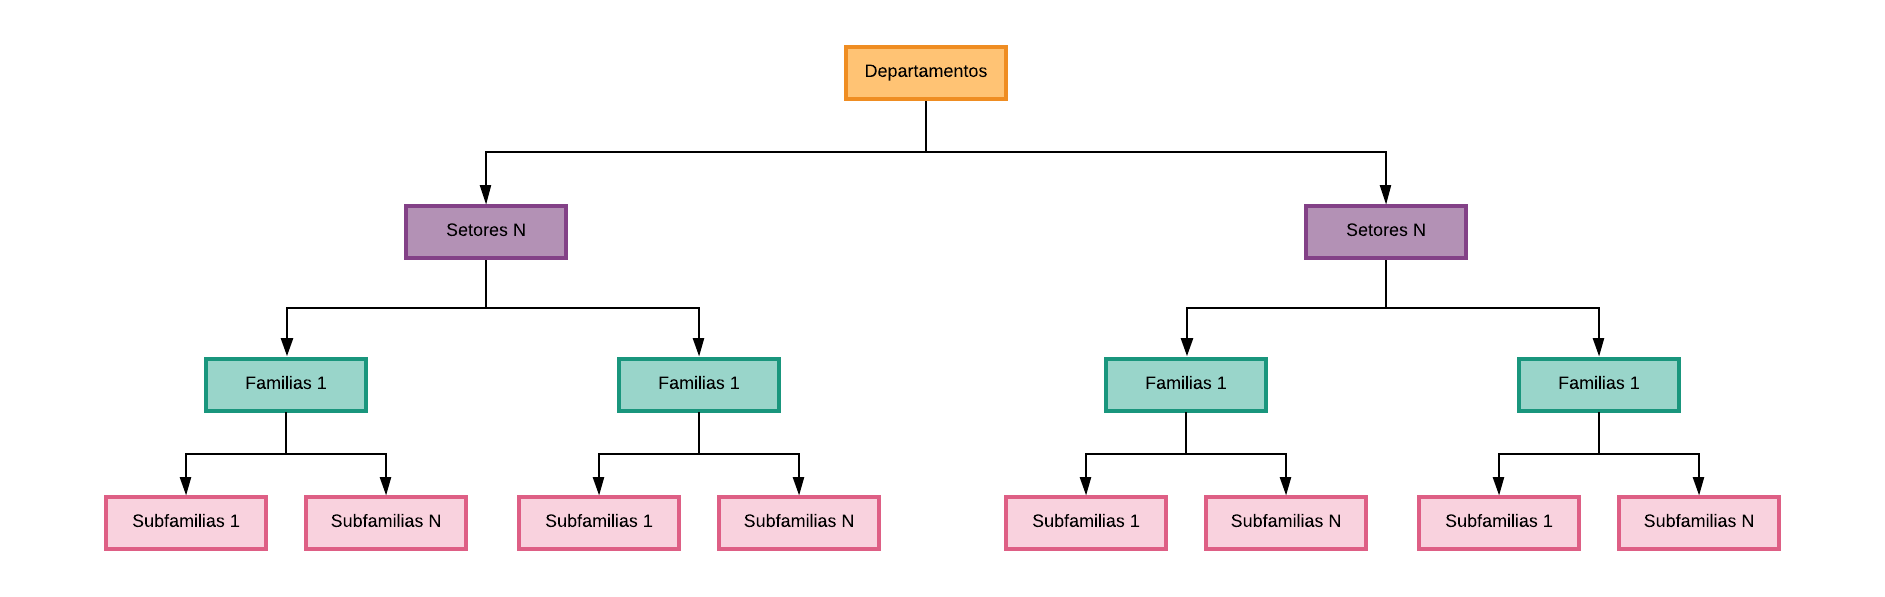
\includegraphics[scale=0.5]{artigo/recursos/imagens/arvore-de-categorias.png}
	\end{center}
	\legend{Fonte: Elaborado pelo Autor}
\end{figure}

\section{PROBLEMAS NOS DADOS}

Como todo conjunto de dados do mundo real, o nosso conjunto de dados não é diferente e possui diversos problemas. Ambiguidades de Categorias, Ruídos e desbalanceamento. A seguir, será feito um resumo dos principais problemas e dificuldades encontrados.

\subsection{AMBIGUIDADES}

A ambiguidade de categorias é outro problema encontrado no nosso conjunto dados, isso de deve a criação desordenada e descentralizada de categorias ao longo dos anos para atender diversos setores da companhia com objetivos distintos. 

\begin{table}[h]
    \centering
    \caption{Amostra de categorias ambíguas no contexto de Mouse para computador}
    \tiny
    \begin{tabularx}{\textwidth}{X|X|X|X} 
        \textbf{DEPARTAMENTO} & \textbf{SETOR} & \textbf{FAMÍLIA} & \textbf{SUBFAMÍLIA} \\ \hline
        INFORMÁTICA ACESSÓRIOS & MOUSE & MOUSE COM FIO & MOUSE COM FIO \\ \hline
        INFORMÁTICA ACESSÓRIOS & MOUSE & MOUSE WIRELESS & MOUSE WIRELESS \\ \hline
        INFORMÁTICA ACESSÓRIOS & MOUSE & MOUSE RETRÁTIL & MOUSE RETRÁTIL \\ \hline
        PC GAMER & MOUSE GAMER & MOUSE COM FIO & MOUSE COM FIO \\ \hline
        PC GAMER & MOUSE GAMER & MOUSE WIRELESS & MOUSE WIRELESS \\ \hline
        PC GAMER & COMBO GAMER & TECLADO E MOUSE & TECLADO E MOUSE \\ \hline
        PC GAMER & COMBO GAMER & MOUSE + MOUSEPAD GAMER & MOUSE + MOUSEPAD GAMER
    \end{tabularx}
    \legend{Fonte: Elaborado pelo autor}
    \label{tab:ambiguidades}
\end{table}

\subsection{RUÍDOS NOS DADOS}

Além dos problemas de ambiguidades, há problemas também de produtos mal categorizados anteriormente, onde por algum equívoco (dificuldade/ambiguidade), um produto foi alocado em uma categoria erroneamente.

Podemos citar um exemplo de que um celular, que poderia estar alocado em televisões. Se este item for selecionado para o treinamento, logo fará com que outros celulares sejam classificados como televisão, um outro problema é uma distorção durante a avaliação dos produtos, pois se esse produto foi selecionado para o conjunto de teste do modelo, logo ele seria classificado como celular, mas a categoria atrelada à ele seria a de televisão.

\subsection{DESBALANCEAMENTO NAS CATEGORIAS}

O problema de desbalanceamento de dados também se encontra presente, para mitigar esse problema utilizamos algumas técnicas como: oversampling, undersampling e  uma função de erro especializada para dados desbalanceados.

\begin{figure}[htb]
	\caption{\label{char_bar_produtos_por_categoria} Quantidade de Produtos Por Departamento}
	\begin{center}
	    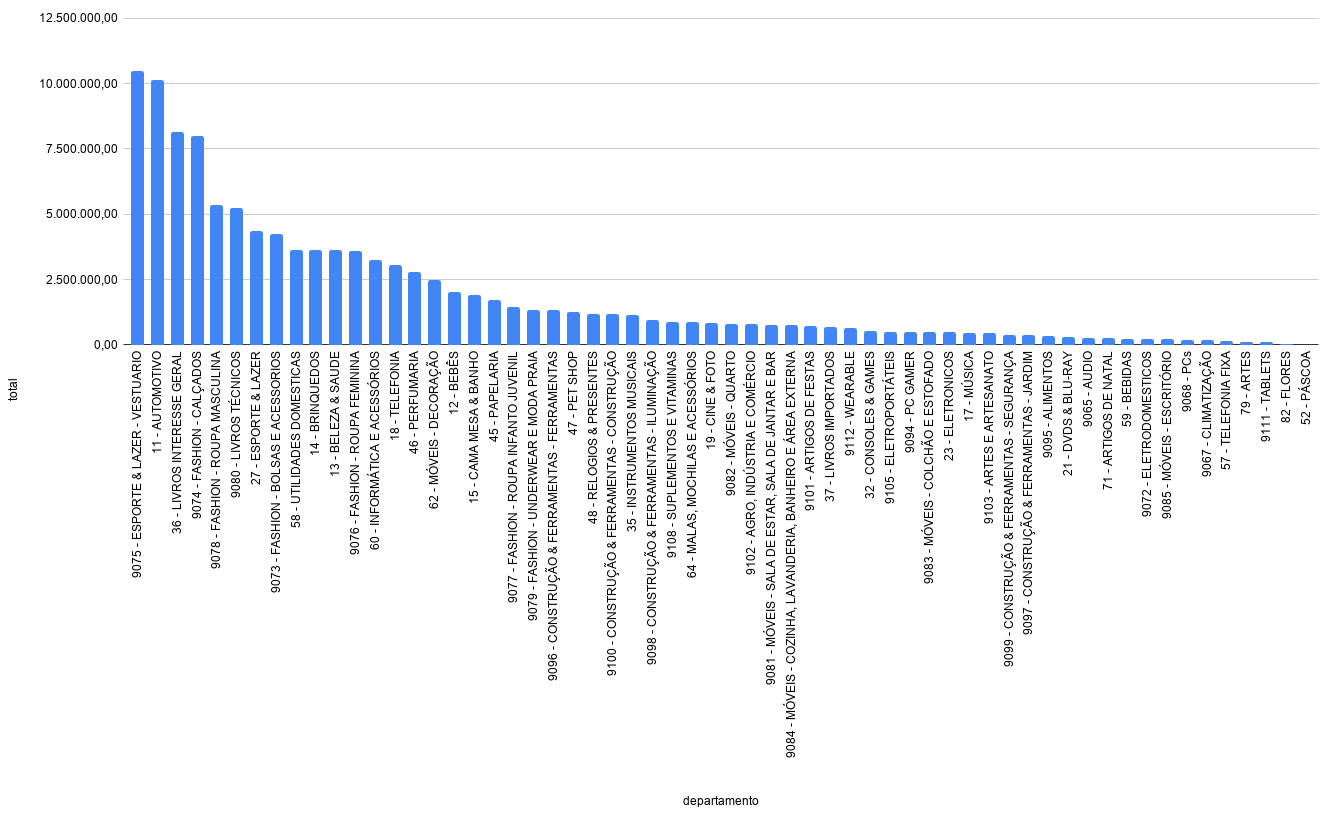
\includegraphics[width=\textwidth]{artigo/recursos/imagens/Quantidade de Produtos por Departamento.png}
	\end{center}
	\legend{Fonte: Elaborado pelo Autor}
\end{figure}

\subsection{LÍNGUA PRÓPRIA}

Os títulos dos produtos são tão distintos nas palavras e na forma de escrever da linguá comum, que partimos do princípio que estamos trabalhando como uma língua distinta de todas as outras. Pois não conseguimos aplicar nenhuma técnica tradicional de Processamento de Linguagem Natural como: lemmantize, stemmer ou mesmo stop-words.

\begin{itemize}
\item Smartphone Samsung Galaxy S10e 128GB Dual Chip Android 9.0 Tela 5,8" Octa-Core 4G Câmera 12MP + 16MP - Preto
\item Geladeira/Refrigerador Electrolux DC35A Branca 260L Cycle Defrost - 220v
\item Tapete Para Sala Shaggy Requinte Casa Dona 100x150cm Cinza
\end{itemize}

É possível observar nos exemplos acima que não seguem nenhuma regra gramatical do português. Além de quê, com a entrada de novos produtos de outros países, presumir regras gramaticais parece imprudente.
\chapter{IMPLEMENTAÇÃO}

O modelo proposto é uma arquitetura de \textbf{Rede Neural Artificial Profunda} com dados heterogêneos não estruturados. Seu formato é a combinação de outras arquiteturas já conhecidas e amplamente utilizadas para resolver separadamente problemas de \textbf{Processamento de Linguagem Natural} e \textbf{Visão Computacional}.

\begin{figure}[htb]
	\caption{\label{arquitetura_macro_do_modelo} Arquitetura Macro do Modelo}
	\begin{center}
	    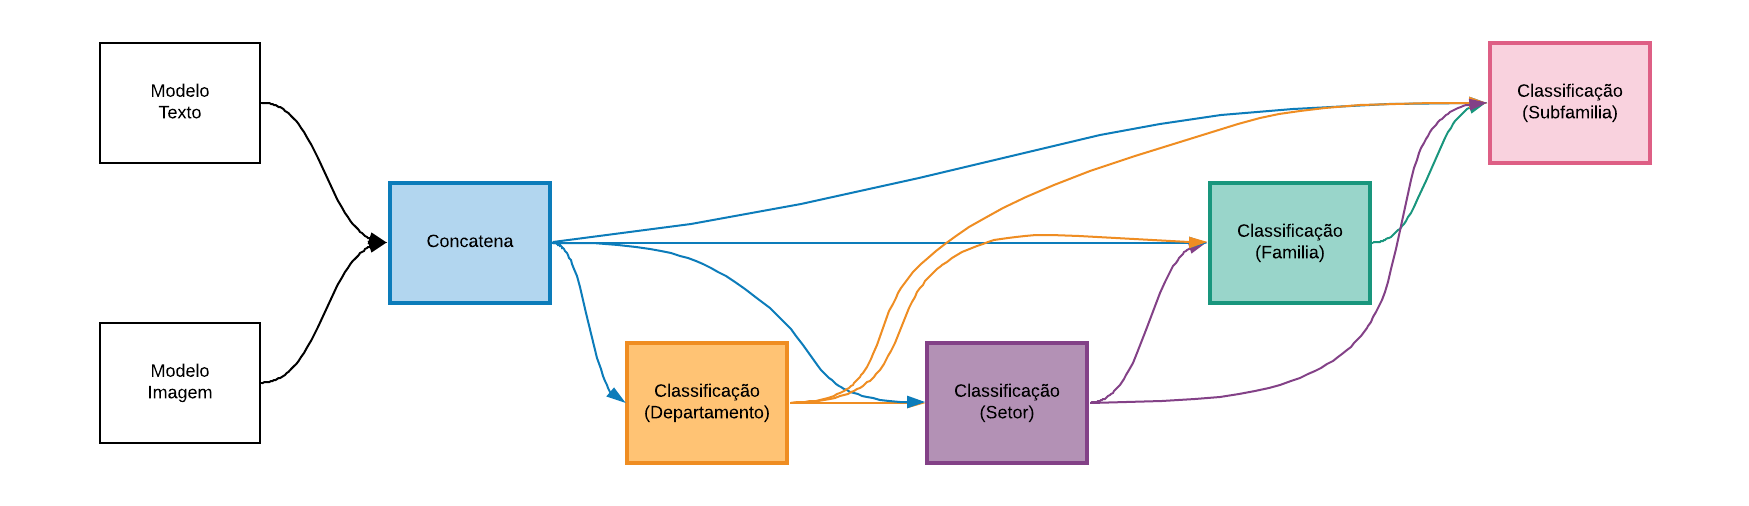
\includegraphics[width=\textwidth]{artigo/recursos/imagens/arquitetura_macro_do_modelo.png}
	\end{center}
	\legend{Fonte: Elaborado pelo Autor}
\end{figure}

Para viabilizar a utilização de dados heterogêneos simultaneamente no modelo, são utilizados dois blocos distintos na rede neural para a extração dos atributos. Para então combinar esses atributos em um conjunto maior que serão injetados nas redes densas de classificação. Vale notar que a saída do nível acima faz parte da entrada do próximo nível.

\section{MODELO DE TEXTO}

O modelo responsável por extrair os atributos dos textos dos produtos, utiliza várias técnicas para atingir este objetivo e pode ser visto na \autoref{modelo_macro_texto}.

\begin{figure}[htb]
	\caption{\label{modelo_macro_texto} Arquitetura Macro do Modelo de texto}
	\begin{center}
	    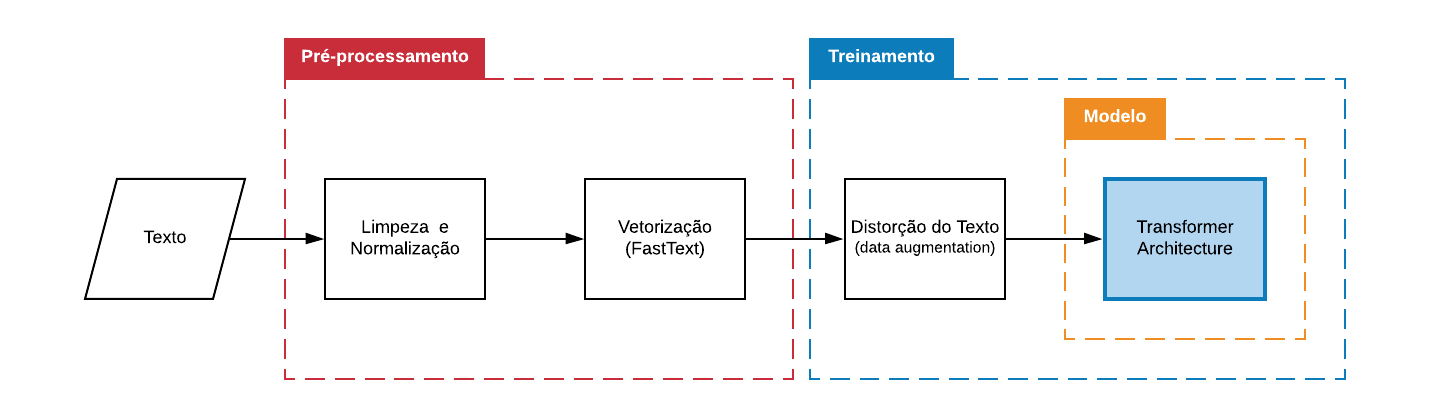
\includegraphics[width=\textwidth]{artigo/recursos/imagens/modelo_macro_texto.png}
	\end{center}
	\legend{Fonte: Elaborado pelo Autor}
\end{figure}

O texto antes do treinamento por \textbf{limpeza e normalização}, \textbf{vetorização} e durante o treinamento o texto recebe \textbf{distorções} em toda interação e então passa pela arquitetura \textbf{Transformer}.

\subsection{LIMPEZA E NORMALIZAÇÃO}

Todo o texto utilizado passa por uma função de limpeza e normalização a fim de remover a maior quantidade de inconsistências e simplificar seu formato. A função de normalização pode ser encontrada no \autoref{chap:funcao_normalizacao_texto}.

\subsection{VETORIZAÇÃO}

A representação do texto de forma vetorial para que possa ser utilizada nos modelos, precisam ser simples e que contenham em si as informações sobre o significado das palavras.

Para o nosso caso, obtivemos melhores resultados usando o \textbf{FasText} proposto no artigo \cite{fasttext}. Esse método de representação vetorial é interessante, pois diferente do \textbf{CBOW} e \textbf{SKIP-GRAM} introduzidos no artigo \cite{mikolov}, o FastText é capaz de representar palavras que não foram vistas durante o treinamento o que é uma grande vantagem no nosso contexto pois muitos termos seguem um padrão de formação, como no exemplo à seguir, onde apenas muda um carácter no modelo do smartphone.

\begin{itemize}
\item Smartphone Samsung Galaxy \textbf{S10} ...
\item Smartphone Samsung Galaxy \textbf{S10e} ...
\item Smartphone Samsung Galaxy \textbf{S10+} ...
\end{itemize}

\subsubsection{REPRESENTAÇÃO DAS PALAVRAS}

As palavras são representadas pela soma da representação vetorial de seus \textit{n-grams} mais um termo especial que é a própria palavra se ela estiver presente no dicionário. Caso a palavra não esteja presente no dicionário, então ela só será representada somente pela soma de seus \textit{n-grams}.

Note que na primeira parte da \autoref{fasttext_representacao_das_palavras_ngram} a palavra “água” aparecer como um termo especial, enquanto na segunda parte o termo especial não aparece, dando a ideia de que não esta presente no dicionário, portanto a representação da palavra será feita somente pelos seus \textit{n-grams}.

\begin{figure}[htb]
	\caption{\label{fasttext_representacao_das_palavras_ngram} Representação das palavras pelos seus n-grams}
	\begin{center}
	    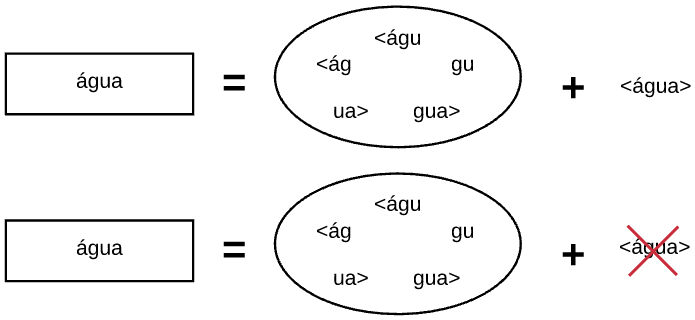
\includegraphics[scale=0.5]{artigo/recursos/imagens/fasttext_representacao_das_palavras_ngram.png}
	\end{center}
	\legend{Fonte: Elaborado pelo Autor}
\end{figure}

Vale notar que o FastText já possui diversos modelos pré-treinados em várias línguas e podem ser encontradas no seu site \href{https://fasttext.cc/docs/en/english-vectors.html}{FastText Models}.

No entanto, para maximizar a performance do modelo, foi necessário fazer um treinamento especializado com os dados do e-commerce. Para mais detalhes, veja o XXXXXXXXXXX.


\begin{center}\large
    $s(w, c) = \sum_{g \in G_w} z_{g}^{T} v_c$
\end{center}

\subsubsection{MODELO FASTTEXT}

O modelo do FastText é uma variação do \textbf{skip-gram} introduzido no \cite{mikolov}, onde dado uma palavra o objetivo é maximizar a probabilidade das palavras em volta. Um exemplo dessa ideia pode ser visto na \autoref{skip_gram_model}.

\begin{figure}[htb]
	\caption{\label{skip_gram_model} SKIP-GRAM Model}
	\begin{center}
	    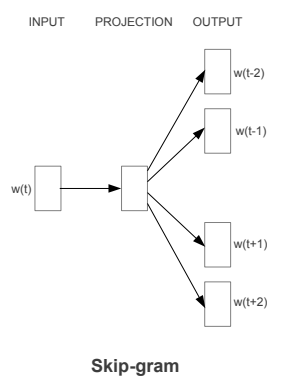
\includegraphics[scale=0.5]{artigo/recursos/imagens/skip_gram_model.png}
	\end{center}
	\legend{Fonte: Disponível em \cite{mikolov}}
\end{figure}

\begin{center}\large
    $\sum_{t=1}^{T} = \left [ \sum_{c \in C_t} l(s(w_t, w_c))) + \sum_{n \in N_{t,c}} l(-s(w_t, n)) \right ]$
\end{center}

\begin{center}\large
    $l(x) = log(1 + e^{-x})$
\end{center}

\subsection{DISTORÇÃO DO TEXTO}

Para tornar o treinamento mais genérico possível e com maior variabilidade dos dados, é utilizado dois tipos de distorção no texto (data augmentation), sendo a primeira a de remover palavras e a segunda de inverter a ordem de palavras de forma randômica e uniforme. As funções que implementam essa funcionalidade estão disponíveis no APÊNDICE - B.

\subsection{ARQUITETURA TRANSFORMER}

É utilizado a arquitetura \textbf{"Transformer"} proposta no artigo \cite{transformer} que é responsável pela a extração dos atributos dos textos.

\begin{figure}[htb]
	\caption{\label{transformer_architecture} Arquitetura Transformer}
	\begin{center}
	    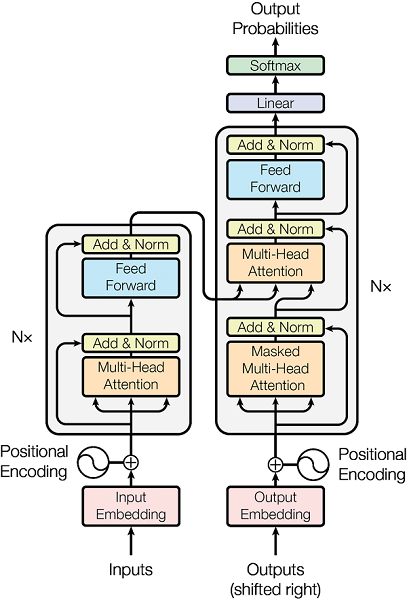
\includegraphics[scale=0.5]{artigo/recursos/imagens/transformer_architecture.png}
	\end{center}
	\legend{Fonte: Disponível em \cite{transformer}}
\end{figure}

A arquitetura é constituída de dois principais blocos. O Codificador (Encoder) e o Decodificador (Decoder) para fazer a tradução de textos. Para o nosso contexto, que é a classificação de produtos, é utilizado somente o bloco \textbf{Codificador} que pode ser visto na \autoref{transformer_bloco_codificador}.

\begin{figure}[htb]
	\caption{\label{transformer_bloco_codificador} Bloco Codificador da Arquitetura Transformer}
	\begin{center}
	    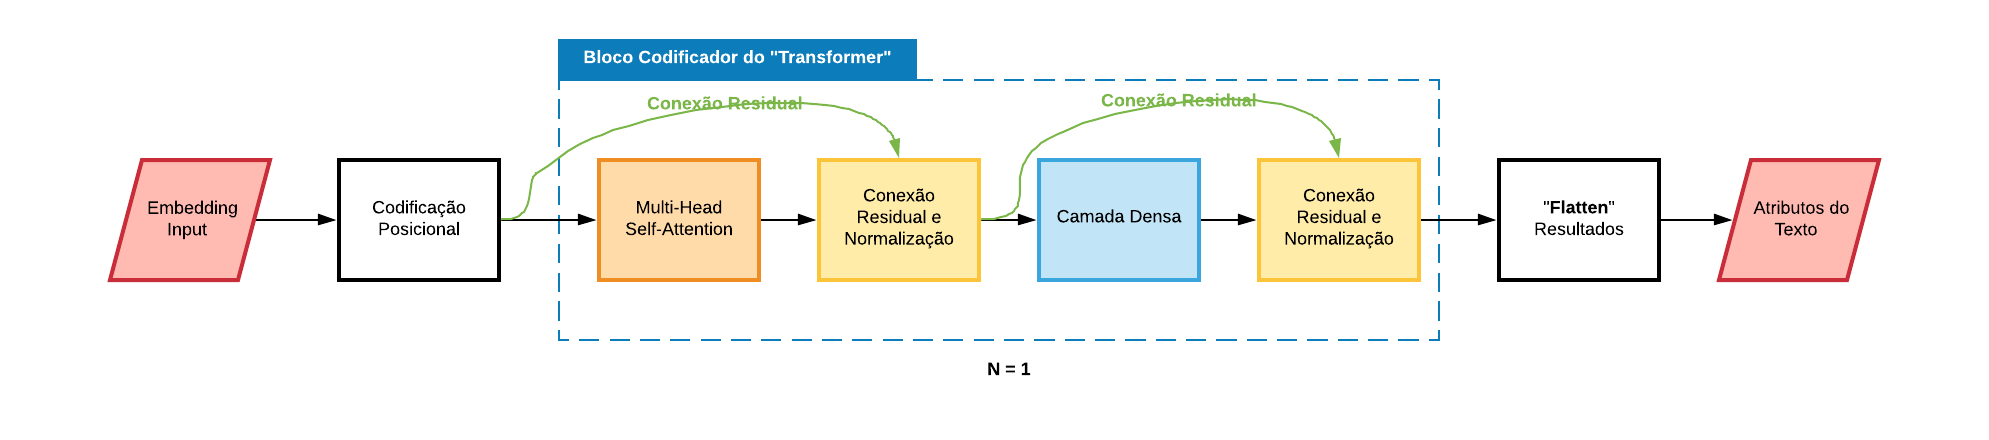
\includegraphics[scale=0.5]{artigo/recursos/imagens/transformer_bloco_codificador.png}
	\end{center}
	\legend{Fonte: Elaborado pelo Autor}
\end{figure}

Vale notar, que na implementação atual, é utilizado somente um bloco do Codificador onde foi possível obter excelentes resultados. Ficando para trabalhos futuros averiguar a necessidade de adicionar mais blocos, criando uma pilha de codificadores.

\subsubsection{EMBEDDING INPUT}

O “embedding Input” é uma (Xijd) sequência vetorial de tamanho pré-definido que é a representação do texto em formato de matriz, onde essa matriz é gerada pelo FastText e então distorcida.

Xi,jd

One i é o tamanho do lote (batch), j é o tamanho da sequência (quantidade de palavras) e d é a quantidade de dimensões do vetor das palavras (tamanho da saído do vetor do FastText). 

O tamanho de j varia conforme o conjunto de dados de treinamento, e busca informar qual o tamanho adequado da quantidade máxima de palavras que será utilizado para formar as sequências removendo as discrepâncias (“outliers”) e reduzindo assim a complexidade do modelo. Essa quantidade é definida à partir de:

%A = {c0 ... cn}| A está ordenada
%k = ⌈p(n+1) / 100⌉

Onde A é uma sequência ordenada da quantidade de palavras por exemplo do conjunto de dados de treinamento,  p-ésimo é a parte  do conjunto de dados que estamos buscando (foi utilizado o valor de p igual à 99,7) e n é o tamanho da amostra, ambos os valores são calculados à partir do conjunto de dados de treinamento. O resultado k é o posição de A que representa a quantidade de palavras que será utilizada.

\subsubsection{CODIFICAÇÃO POSICIONAL}

Nesta etapa, o objetivo é adicionar a informação de posição nas sequências. Isso se faz necessário, pois o modelo não possui consciência do que é posição, diferente de uma Rede Neural Recorrente. A função para a codificação das sentenças se dá por:

Onde d é o tamanho do vetor dos palavras da sequências e i é um vetor de tamanho d que representa as posições de cada atributo do vetor de palavras.

Enquanto pos é uma matriz do tamanho do l,m onde l é o tamanho do lote e m é a quantidade de palavras na sequência.

Um exemplo do código que faz essa implementação pode ser visto no APÊNDICE X - CODIFICAÇÃO POSICIONAL.

\subsubsection{MULTI-HEAD SELF-ATTENTION}
O que é Attention

A definição de Mecanismo de Atenção (“Attention Mechanism”) consiste em “Each annotation hi contains information about whole input sequence with a strong focus on the partes surrounding the i-th word of the input sequence” de acordo com [2], em tradução direta “Cada anotação hi contém informação sobre toda a sentença, com ênfase nas partes que rodeiam a palavra i-th da sequência de entrada”.

É possível observar que a ideia consiste em em criar um contexto para cada palavra na sequência onde determinadas palavras têm mais relevância do que outras.

Onde o contexto ci é criado pelo somatório do produto dos pesos aij com as palavras. Onde os pesos são calculados para todas as palavras usando a função softmax.

O que é self attention

o que Multi-Head self-attention


\subsubsection{CONEXÃO RESIDUAL E NORMALIZAÇÃO}
asdsad

\subsubsection{CAMADA DENSA}
asdasd


\section{IMAGEM}

Para a extração dos atributos das imagens é utilizado o modelo da ResNet proposto no artigo \cite{resnet} além das imagens passarem por distorções em cada nova interação. O formato da estada das imagens é no formato \textbf{RGB 64x64x3}.

\begin{figure}[htb]
	\caption{\label{modelo_imagem_macro} Arquitetura do modelo de Imagem}
	\begin{center}
	    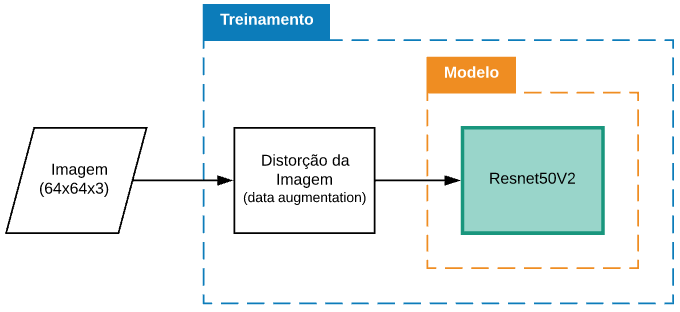
\includegraphics[scale=0.5]{artigo/recursos/imagens/modelo_imagem_macro.png}
	\end{center}
	\legend{Fonte: Elaborado pelo Autor}
\end{figure}


\subsection{DISTORÇÃO DAS IMAGENS}

Assim como foi feito nos textos, também é feito a distorção (data augmentation) nas imagens para tornar o treinamento melhor e mais genérico, pois toda vez que uma imagem passa pela rede, é como se fosse uma nova imagem. Para atingir esse objetivo é empregado diversas modificações nas imagens como pode ser visto no exemplo na \autoref{imagem_distorcao} e no \autoref{chap:funcao_distorcao_imagem} pode ser encontrado a implementação.

\begin{figure}[htb]
	\caption{\label{imagem_distorcao} Distorção de Imagem}
	\begin{center}
	    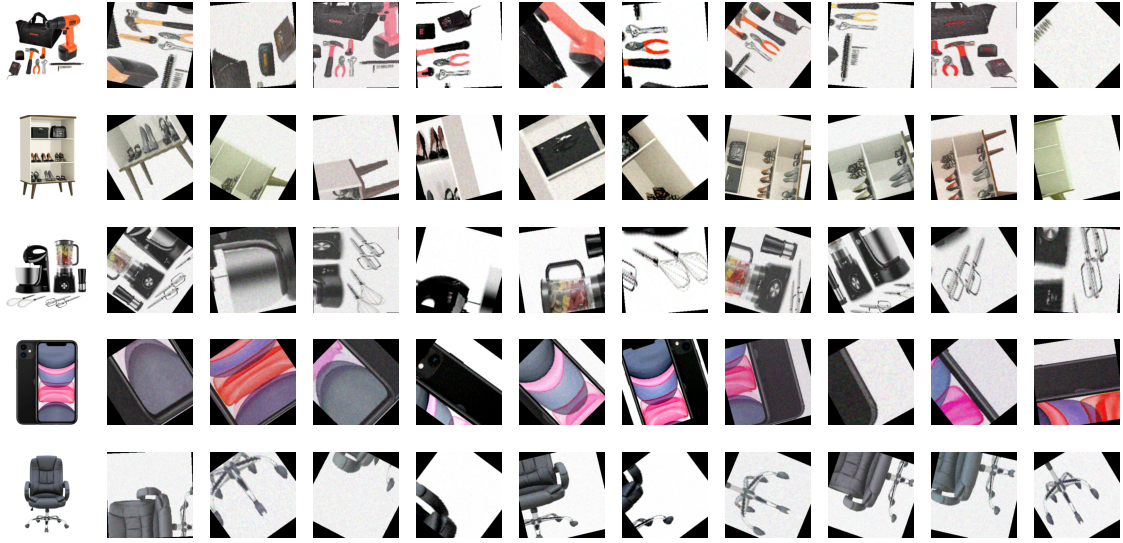
\includegraphics[width=\textwidth]{artigo/recursos/imagens/imagem_distorcao.png}
	\end{center}
	\legend{Fonte: Elaborado pelo Autor}
\end{figure}

\subsection{ARQUITETURA RESNET V2}

Como arquitetura para a extração de features é utilizado a ResNet V2 

\section{CONJUNTO DE DADOS}
Como não há uma possibilidade no momento de criar um conjunto de dados anotados manualmente, utilizamos os produtos já classificados previamente.     Com isso, o conjunto de dados é separado em três partes:

conjunto de dados de treinamento (inclui técnica de oversampling e undersampling)
conjunto de dados de validação (utilizado para acompanhar a performance do modelo durante o treinamento é usado na cláusula de parada)

conjunto de dados de teste (utilizado para criar o relatório final)

\subsection{SELEÇÃO DO CONJUNTO DE DADOS}

Para tentar criar um conjunto de dados razoável, precisamos tomar como premissa de que os dados que possuímos estão corretos e são aplicados as seguintes técnicas:

Para tentar reduzir o ruído no conjunto de dados, é utilizado um modelo de auxiliar capaz de identificar possíveis produtos mal categorizados;

Quanto os produtos de uma subfamília possuem quantidade menor ou igual à 3, essas subfamílias são removidas pois não possuem dados o suficiente para treinar, validar e testar;

Uma vez o conjunto de dados selecionado, é feito a separação dos dados de treinamento, validação e teste. Onde 90 dos dados são para treinamento, 5 para validação e 5 para teste. Os dados de treinamento passam ainda por oversampling e undersampling.
Para as subfamílias com muitos produtos, são feitas o undersampling definindo um máximo de a Média mais duas vezes o Desvio padrão (mean + 2*std);
Para as subfamílias com produtos menores que 30, é feito o oversampling (replicação de exemplos) até ficarem com 30 amostras.

\section{TREINAMENTO}

O treinamento do modelo ocorre utilizando 8 GPUs Nvidia V100 durante X dias e para somente baseado na cláusula de parada que pode ser visto na seção 2.4.3 CLÁUSULA DE PARADA. 

\subsection{OTIMIZADOR}

Para o otimizador é utilizado mini-batch (128) com SGD com Momentum e Nesterov a fim de aumentar a velocidade do treinamento com o learning rate inicial de 0,01 e sendo reduzido após a décima época num fator exponencial.

\subsection{FUNÇÃO DE ERRO (LOSS FUNCTION)}

Como os dados são extremamentes desbalanceados e em certas classes tem tão poucos e outras grandes quantidades de exemplos e a variabilidade e sutileza, buscamos na literatura uma função de erro que fosse capaz de incluir esse desbalanceamento durante o treinamento.
O Focal Loss é uma variação do Cross Entropy especializado em dados desbalanceados desenvolvido para detectar objetos sob fundos em imagens. Foi desenvolvido no Facebook AI Research (LIN et al., 2017). A publicação esta disponível em: https://arxiv.org/abs/1708.02002 e o código fonte de exemplo está disponível no APÊNDICE C.
ADICIONAR FUNÇÃO MATEMÁTICA

\subsection{CLÁUSULA DE PARADA}

É definido como cláusula de parada, quando o modelo para de conseguir reduzir o loss do conjunto de dados de validação com uma paciência de 10 épocas.


\phantompart

% ----------------------------------------------------------
% ELEMENTOS PÓS-TEXTUAIS
% ----------------------------------------------------------
\postextual

% ----------------------------------------------------------
% Referências bibliográficas
% ----------------------------------------------------------
\bibliography{sample.bib}

% ----------------------------------------------------------
% Glossário
% ----------------------------------------------------------
%
% Consulte o manual da classe abntex2 para orientações sobre o glossário.
%
%\glossary

% ----------------------------------------------------------
% Apêndices
% ----------------------------------------------------------

% ---
% Inicia os apêndices
% ---
\begin{apendicesenv}

% Imprime uma página indicando o início dos apêndices
\partapendices
\clearpage
\clearpage

\chapter{FUNÇÃO DE NORMALIZAÇÃO DE TEXTO}
\label{chap:funcao_normalizacao_texto}

O código pode ser acessado no repositório do projeto em:
\url{https://github.com/allanbatista/classificacao-de-produtos-no-e-commerce/blob/master/codigo/notebooks/Cleaner.ipynb}.


\chapter{FUNÇÃO DE DISTORÇÃO DE TEXTO}
\label{chap:funcao_distorcao_texto}

O código pode ser acessado no repositório do projeto em:
\url{https://github.com/allanbatista/classificacao-de-produtos-no-e-commerce/blob/master/codigo/notebooks/Distor\%C3\%A7\%C3\%A3o_de_Texto.ipynb}.

\clearpage
\chapter{FUNÇÃO DE DISTORÇÃO DE IMAGEM}
\label{chap:funcao_distorcao_imagem}

O código pode ser acessado no repositório do projeto em 
\url{https://github.com/allanbatista/classificacao-de-produtos-no-e-commerce/blob/master/codigo/notebooks/Distor\%C3\%A7\%C3\%A3o_de_Imagens_com_Tensorflow.ipynb}.

\chapter{FASTTEXT MODELO PRÉ-TREINADO}
\label{chap:fasttext_modelo_pretreinado}


\section{Configurações do Treinamento}

\begin{table}[htb]
    \ABNTEXfontereduzida
    \centering
    \caption[Configurações de Treinamento do FastText]{Configurações de Treinamento do FastText.}
    \begin{tabular}{|r|l|} \hline
        epocas & 50 \\ \hline
        dimensão & 128 \\ \hline
        n-grams & 1 até 3 \\ \hline
        n-grams por palavra & 2 até 7 \\ \hline
        tamanho do dicionário & 5000000 \\ \hline
    \end{tabular}
    \legend{Fonte: Elaborado pelo Autor}
    \label{tab:fasttext_configuracores}
\end{table}

\section{Modelos Pré-Treinados}

Modelo do FasText: \url{https://storage.googleapis.com/black-magic-us-west1/fasttext/2020-07-16T00-00-00/model.bin}

Modelo Embeddins das palavras: \url{https://storage.googleapis.com/black-magic-us-west1/fasttext/2020-07-16T00-00-00/model.vec}

\section{Corpus}

\begin{simpletext}\small
\url{https://storage.googleapis.com/black-magic-us-west1/fasttext/2020-07-16T00-00-00/000000000000.txt} \\
\url{https://storage.googleapis.com/black-magic-us-west1/fasttext/2020-07-16T00-00-00/000000000001.txt} \\
\url{https://storage.googleapis.com/black-magic-us-west1/fasttext/2020-07-16T00-00-00/000000000002.txt} \\
\url{https://storage.googleapis.com/black-magic-us-west1/fasttext/2020-07-16T00-00-00/000000000003.txt} \\
\url{https://storage.googleapis.com/black-magic-us-west1/fasttext/2020-07-16T00-00-00/000000000004.txt} \\
\url{https://storage.googleapis.com/black-magic-us-west1/fasttext/2020-07-16T00-00-00/000000000005.txt} \\
\url{https://storage.googleapis.com/black-magic-us-west1/fasttext/2020-07-16T00-00-00/000000000006.txt} \\
\url{https://storage.googleapis.com/black-magic-us-west1/fasttext/2020-07-16T00-00-00/000000000007.txt} \\
\url{https://storage.googleapis.com/black-magic-us-west1/fasttext/2020-07-16T00-00-00/000000000008.txt} \\
\url{https://storage.googleapis.com/black-magic-us-west1/fasttext/2020-07-16T00-00-00/000000000009.txt} \\
\url{https://storage.googleapis.com/black-magic-us-west1/fasttext/2020-07-16T00-00-00/000000000010.txt} \\
\url{https://storage.googleapis.com/black-magic-us-west1/fasttext/2020-07-16T00-00-00/000000000011.txt} \\
\url{https://storage.googleapis.com/black-magic-us-west1/fasttext/2020-07-16T00-00-00/000000000012.txt} \\
\url{https://storage.googleapis.com/black-magic-us-west1/fasttext/2020-07-16T00-00-00/000000000013.txt} \\
\url{https://storage.googleapis.com/black-magic-us-west1/fasttext/2020-07-16T00-00-00/000000000014.txt} \\
\url{https://storage.googleapis.com/black-magic-us-west1/fasttext/2020-07-16T00-00-00/000000000015.txt} \\
\url{https://storage.googleapis.com/black-magic-us-west1/fasttext/2020-07-16T00-00-00/000000000016.txt} \\
\url{https://storage.googleapis.com/black-magic-us-west1/fasttext/2020-07-16T00-00-00/000000000017.txt} \\
\url{https://storage.googleapis.com/black-magic-us-west1/fasttext/2020-07-16T00-00-00/000000000018.txt} \\
\url{https://storage.googleapis.com/black-magic-us-west1/fasttext/2020-07-16T00-00-00/000000000019.txt}
\end{simpletext}

\chapter{CODIFICAÇÃO POSICIONAL}
\label{chap:transformer_codificao_posicional}

O código pode ser acessado no repositório do projeto em \url{https://github.com/allanbatista/classificacao-de-produtos-no-e-commerce/blob/master/codigo/notebooks/Transformer_Codificacao_Posicional.ipynb}.

\chapter{FOCAL LOSS}
\label{chap:focal_loss}

O código pode ser acessado no repositório do projeto em \url{https://github.com/allanbatista/classificacao-de-produtos-no-e-commerce/blob/master/codigo/notebooks/Focal_Loss_for_Dense_Object_Detection.ipynb}.


\end{apendicesenv}


% ----------------------------------------------------------
% Anexos
% ----------------------------------------------------------

% ---
% Inicia os anexos
% ---
\begin{anexosenv}

% Imprime uma página indicando o início dos anexos
\partanexos

% ---
\chapter{Exemplo Anexo}
% ---
\lipsum[30]


\end{anexosenv}

%---------------------------------------------------------------------
% INDICE REMISSIVO
%---------------------------------------------------------------------

\phantompart

\printindex

\end{document}
